%\documentclass[aps,prl,twocolumn,showpacs,superscriptaddress,groupedaddress]{revtex4}
%% for review and submission
%\documentclass[aps,preprint,showpacs,superscriptaddress,groupedaddress]{revtex4}
% for double-spaced preprint
%\documentclass[aps,prl,floatfix,twocolumn,10pt]{revtex4-1}
%for review and submission
\documentclass[aps,prl,preprint,english]{revtex4-1} 
% for double-spaced preprint
%\documentclass[aip,apl,amsmath,amssymb,floatfix,preprint,a4paper]{revtex4-1}
%\documentclass[aip,apl,amsmath,amssymb,floatfix,reprint,a4paper]{revtex4-1}

%% Packages
\usepackage[T1]{fontenc}
\usepackage[utf8]{inputenc} %Umlaute
\usepackage{babel}
\usepackage{acronym}
\usepackage{amsmath}
\usepackage{amssymb}
\usepackage[bf,small,labelsep=period]{caption}
\usepackage{graphicx}  %figures
\usepackage[detect-all]{siunitx}

\addto\captionsenglish{\renewcommand{\figurename}{Figure}}
%% New commands
\newcommand{\msub}[1]{\ensuremath{\textnormal{\begin{tiny}#1\end{tiny}}}}
\renewcommand{\d}[1]{\ensuremath{\operatorname{d}\!{#1}}}
\DeclareSIUnit{\voltpeak}{Vp}

%acronyms
\acrodef{CT}{computed tomography}
\acrodef{SNR}{signal-to-noise ratio}
\acrodef{CNR}{contrast-to-noise ratio}
\acrodef{SEM}{scanning electron microscope}
%% ----------------------------------------------------------------------------------------------------------------

\begin{document}

\title{X-ray phase-contrast imaging at \SI{100}{\kilo\electronvolt} on
conventional sources}

\author{T.~Thüring}
\affiliation{Paul Scherrer Institute, Villigen PSI, Switzerland}
\affiliation{Institute for Biomedical Engineering, Swiss Federal Institute of Technology, Zurich, Switzerland}
\author{M.~Abis}
\affiliation{Paul Scherrer Institute, Villigen PSI, Switzerland}
\affiliation{Institute for Biomedical Engineering, Swiss Federal Institute of Technology, Zurich, Switzerland}
\author{Z.~Wang}
\affiliation{Paul Scherrer Institute, Villigen PSI, Switzerland}
\author{C.~David}
\affiliation{Paul Scherrer Institute, Villigen PSI, Switzerland}
\author{M.~Stampanoni}
\affiliation{Paul Scherrer Institute, Villigen PSI, Switzerland}
\affiliation{Institute for Biomedical Engineering, Swiss Federal Institute of Technology, Zurich, Switzerland}

\date{\today}


%% ----------------------------------------------------------------------------------------------------------------
\begin{abstract}
    X-ray grating interferometry is a promising imaging technique sensitive
    to attenuation, refraction and scattering of the radiation. Applications
    of this technique in the energy range between $80$ and
    $\SI{150}{\kilo\electronvolt}$ are still largely unexplored due to the
    severe technical challenges. Phase-contrast X-ray imaging at such high
    energies is of relevant scientific and industrial interest, in
    particular for the investigation of materials with high atomic number or
    thickness as well as for medical imaging. Here we show the successful
    implementation of a Talbot-Lau interferometer operated at
    $\SI{100}{\kilo\electronvolt}$ using a conventional X-ray tube and a
    compact geometry, with a total length of $\SI{54}{\centi\metre}$. We
    present edge-on illumination of the gratings to overcome their current
    fabrication limits as well as curved structures, to match beam
    divergence and allow large field of views on a short and efficient
    setup.
\end{abstract}
\maketitle

%%%%%%%%%%%%%%%%%%%%%%%%%%%%%%%%%%%%%%%%%%%%%%%%%%%%%%%%%%%%%%%%%%%%%%%%
% Body of manuscript
%%%%%%%%%%%%%%%%%%%%%%%%%%%%%%%%%%%%%%%%%%%%%%%%%%%%%%%%%%%%%%%%%%%%%%%%

X-ray radiography and \ac{CT} are standard imaging techniques in
materials and life sciences for the nondestructive examination of samples or
diagnostic tasks in medicine. The underlying contrast mechanism
relies on the different X-ray attenuation properties of different materials
or tissue types. The dominant physical effects contributing to attenuation
are the photoelectric effect and incoherent (Compton) scattering. Besides attenuation, the wave
nature of X-rays reveals another contrast mechanism, which is the phase
shift. The interaction contributing to phase shifts is coherent (Rayleigh)
scattering~\cite{Als-Nielsen2011}.

The attenuation and phase shift properties are described by the complex index of refraction
$n=1-\delta + i \beta$.
The imaginary part $\beta$ is related to the
attenuation coefficient by $\mu = 4 \pi
\beta(\lambda) / \lambda$, while the real part
$\delta(\lambda)$ determines the phase shift 
$\phi = 2 \pi \delta(\lambda) / \lambda$

While the attenuation can be measured with an
X-ray detector as the reduction of the beam intensity, the phase
is not directly observable. Therefore, an optical system is needed to
convert the phase shift into intensity modulations.

Phase-sensitive
imaging is a desirable modality, as it delivers a complementary source of
contrast with respect to absorption by providing direct access 
to the electron density~\cite{Als-Nielsen2011}. Moreover, the combination with
attenuation enables the determination of the effective atomic
number~\cite{Qi2010}.
An enhanced
\ac{CNR} in images compared to attenuation for certain
materials or tissues~\cite{Pfeiffer2007a,McDonald2009} has also been
demonstrated.

The vast majority of phase-sensitive techniques, including crystal analyzer
based~\cite{Davis1995,Chapman1997} or interferometric~\cite{Bonse1965,Momose1996}
methods rely on X-ray beams of high spatial and temporal coherence, which is
available only at synchrotron sources. Inline
phase contrast~\cite{Snigirev1995,Wilkins1996,Cloetens1996} and
Talbot interferometry~\cite{Cloetens1997,David2002,Momose2003a} need high
spatial coherence but are available on polychromatic microfocus sources.
Phase-contrast imaging using X-ray beams of low temporal \emph{and}
spatial coherence such as conventional low-brilliance X-ray tubes have been
demonstrated with coded
apertures~\cite{Munro2012} and Talbot-Lau
interferometry~\cite{Pfeiffer2006}. Analyzer-based systems have been
recently extended to tube sources~\cite{Nesch2009,Parham2009}
but only at energies up
to the tungsten $K_\alpha$ line at~\SI{60}{\kilo\eV}.
In addition to phase sensitivity, analyzer-based, Talbot interferometry and
coded-aperture approaches also provide (with different retrieval mechanisms)
information about the integrated local small angle scattering power from
microscopic density fluctuations in a specimen~\cite{Pfeiffer2008}. This signal is known under the name of dark-field, scatter or visibility reduction contrast.

High-energy Talbot interferometry has been reported so far using a
synchrotron source at nominal energies of
$\SI{82}{\kilo\electronvolt}$~\cite{Willner2013} and 
$\SI{123}{\kilo\electronvolt}$~\cite{Ruiz2013}.
Using a low-brilliance X-ray tube, Talbot-Lau interferometry was
applied so far at $\SI{60}{\kilo\electronvolt}$ mean energy~\cite{Donath2009}.
Medical imaging applications may benefit from phase contrast at higher
energies: chest or abdominal
radiography or \ac{CT} require energies between $100$ and
$\SI{150}{\kilo\voltpeak}$. Other potential applications are homeland
security or chip failure analysis, which require high energies for the
visualization of materials of high density and atomic number.

Here we introduce a method for phase contrast imaging which works on
conventional X-ray sources, covers the entire diagnostic X-ray energy range
and is compatible with compact imaging arrangements. The approach is based
on
Talbot-Lau
interferometry~\cite{Pfeiffer2006} and employs an edge-on illumination approach for the grating design and
arrangement. 
Our solution removes one on the major hurdle which prevented grating interferometry to be applied at very high X-ray energies so far, namely the fabrication of gratings with high-aspect ratios.
 The aspect
ratio, given by
\begin{equation}
    \text{R} = \frac{2h}{p},
\end{equation}
where $p$ is the grating period and $h$ the  structure
height, is normally limited by the fabrication process, usually
photolithography~\cite{David2002} or X-ray lithography~\cite{Mohr2012} as grating
structures tend to collapse or deform (e.g. due to capillary forces) if
the aspect ratio is too high. For a given setup length these parameters
depend on the target energy $E$ according to $p \propto
1/\sqrt{E}$ and $h \propto E^3$, and therefore $\textnormal{R}
\propto E^{7/2}$~\cite{Momose2003a}. If at $E=\SI{25}{\kilo\electronvolt}$ an aspect ratio
for the absorption grating around $\textnormal{R}=30$ is necessary for a
reasonable length of the experimental arrangement, it would have to be at
least $128$ for $E=\SI{100}{\kilo\electronvolt}$. Moreover, when using a
broad spectrum, photons above the design energy should also be
efficiently blocked by the gratings, which requires even higher aspect ratios.
The largest aspect ratios achieved by current fabrication techniques~\cite{David2007,Kenntner2010} are around 60.

Our design introduces the edge-on
illuminated,  circularly aligned structures. Edge-on illumination
(figure~\ref{Fig:schematic}), as
opposed to face-on illumination, exploits the dimension along the grating
lines to form a high aspect ratio of the structures in the direction of the beam. The
effective structure height of the grating is then determined by the grating
dimension along the grating lines, which essentially allows arbitrarily high
aspect ratios. 
\begin{figure}[ht]
    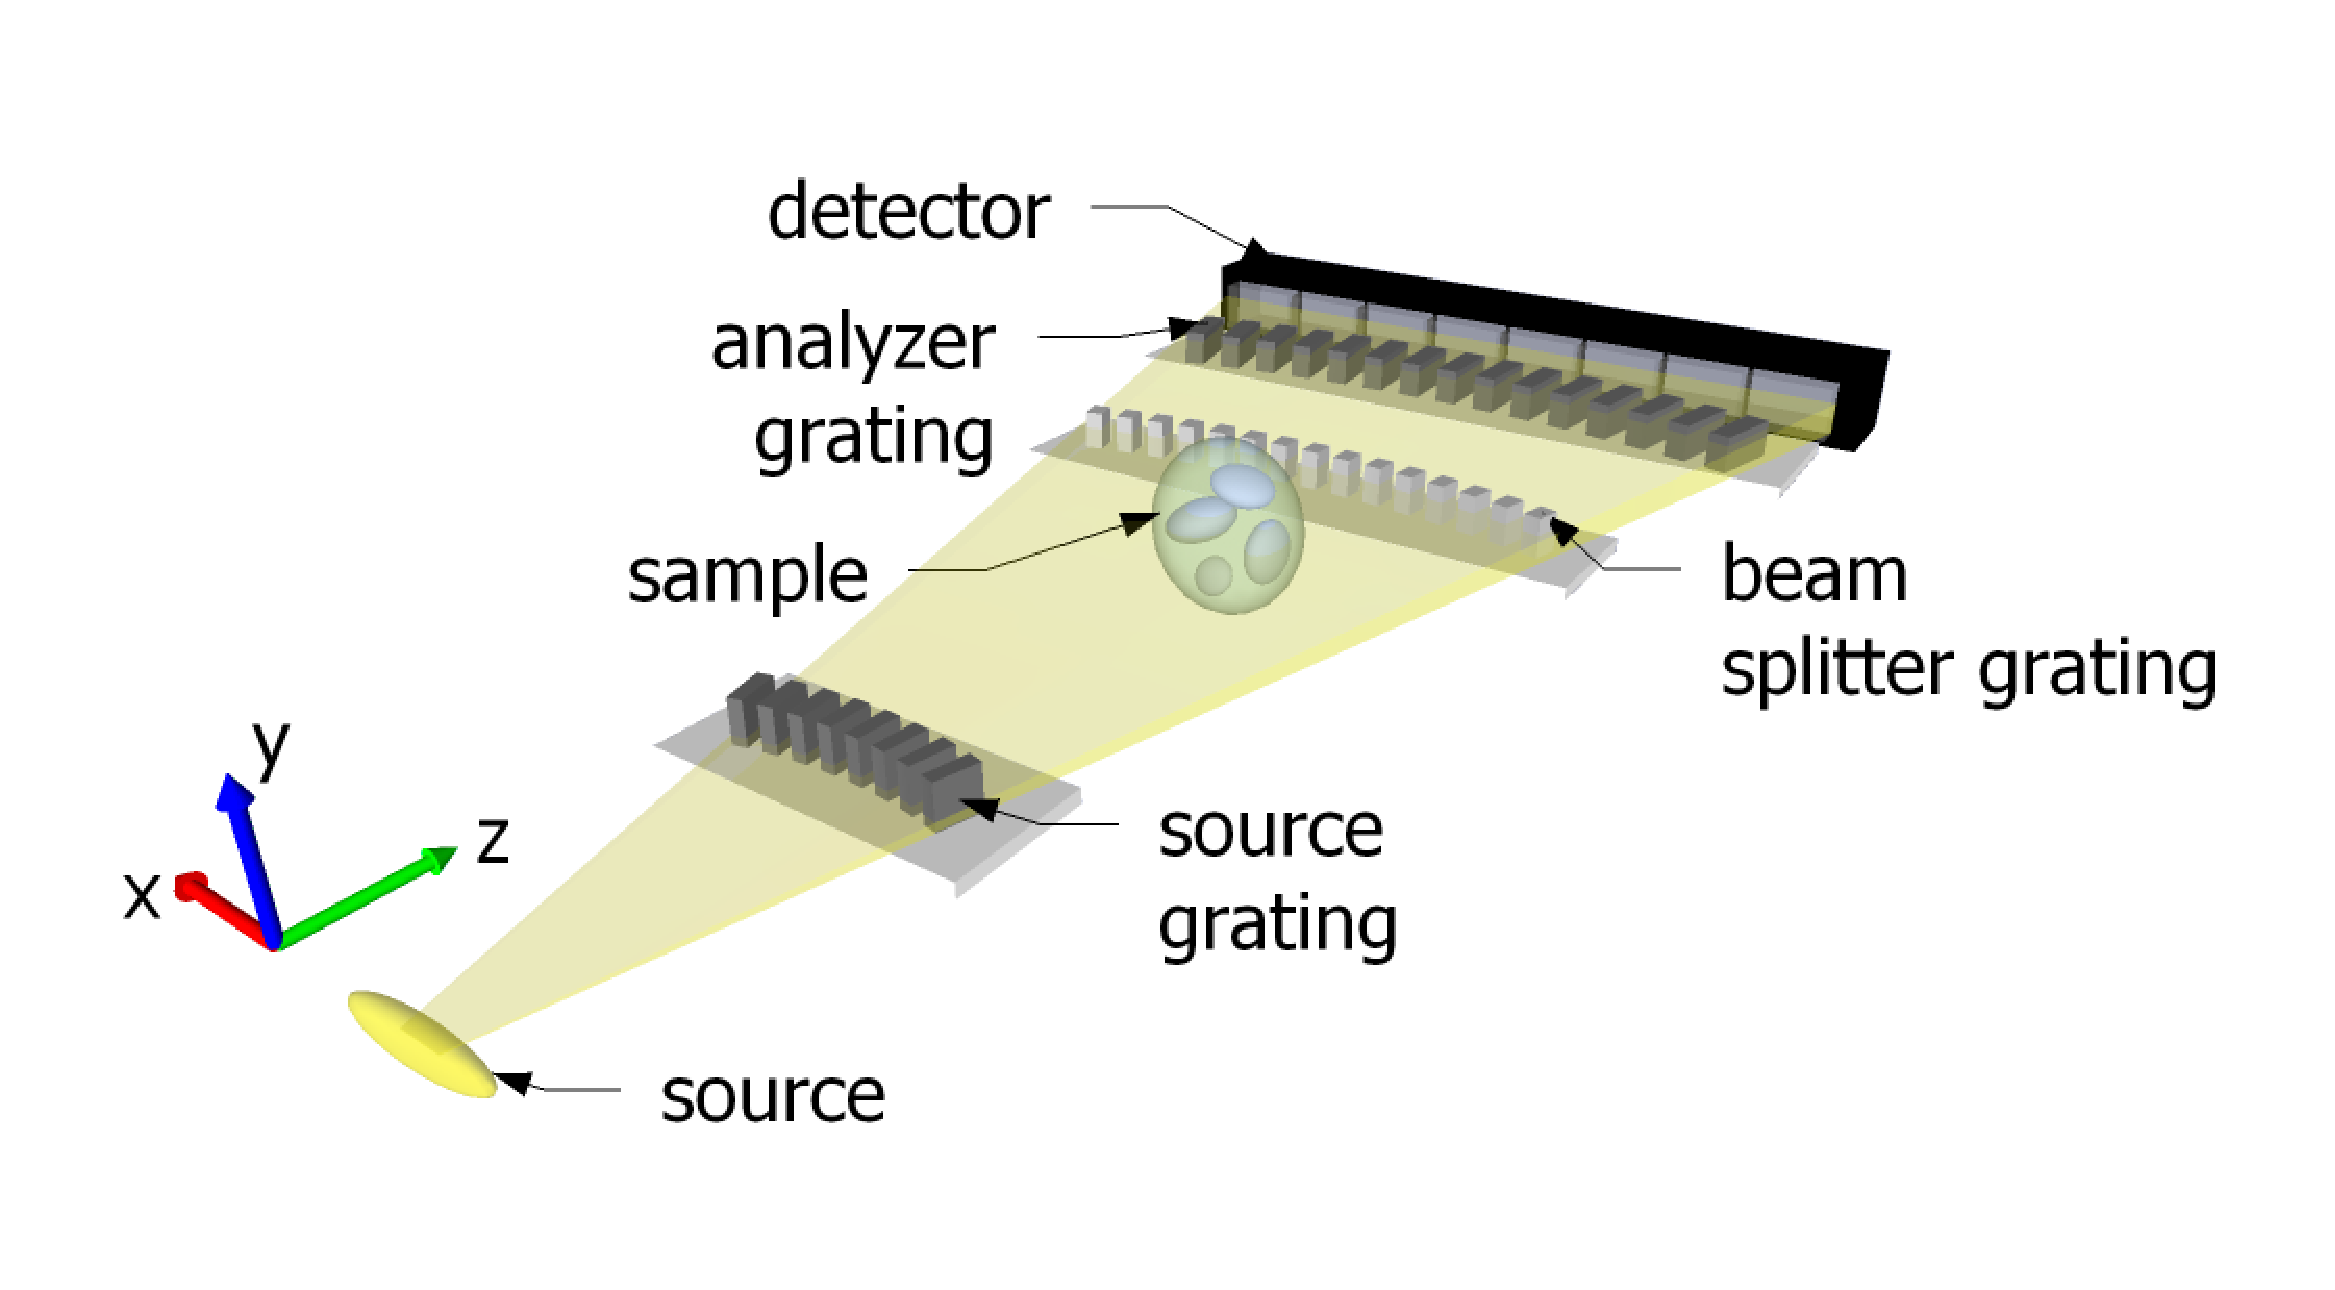
\includegraphics[width=.7\textwidth]{figures/figure1.eps}
    \caption{Schematic of a grating
        interferometer for X-ray energies between 60 and
        \SI{150}{\kilo\electronvolt} in edge-on illumination mode. The
        aspect ratio is defined by the ratio of the travelling distance along the
        grating lines and the period and can be arbitrarily long. In order to avoid
        a reduction of the field of view, the grating structures are aligned on an
    arc.}
    \label{Fig:schematic}
\end{figure}

Increasing the aspect ratio of the gratings typically leads to a
reduction of the field of view due to the change of the grating transmission
function at high incident angles. In order to overcome this problem, the grating lines are circularly aligned 
with a radius equal to the distance to the source. This cannot be done with
the glancing angle approach~\cite{Stutman2012a}, and allows an arbitrarily
large field-of-view in a fan beam geometry.

The combination of edge-on illumination and circularly aligned structures
enables phase-contrast imaging at arbitrary design energies and with a
maximum field of view in the horizontal direction ($x$ direction). These
advantages come at the expense of a limited field of view in the vertical
direction ($y$ direction), which is, depending on the X-ray detector,
typically a few pixels. 
Radiographic 2D imaging can be obtained by scanning the sample or a thin fan
beam. The scanning technique has been demonstrated to deliver less dose than
the conventional approach based on the illumination of a large area. In
digital mammography, for instance, where dose is a critical issue, Philips'
MicroDose system combines a scanning approach with an highly collimated fan
beam~\cite{Aslund2007}. Thanks to the high collimation, the dose deposited
on  patients has been reported to be significantly lower than with other
instruments based on the illumination of a large area
detector~\cite{Oduko2010}.
Similarly, for tomographic images,
the approach allows single slice \ac{CT} or full 3D imaging in scanning mode.

Grating design and fabrication is nonstandard and involves a complex mask
design, as shown in Figure~\ref{Fig:grating_mask}. Multiple gratings can reside on a
silicon chip with their specific structure length and curvature. For the
current experiments, a symmetric interferometer with a grating period of $p
= \SI{2.8}{\micro\metre}$ for all gratings has been used. The design energy
is $\SI{100}{\kilo\electronvolt}$ and the beam splitter grating periodically
shifts the phase by zero and $\pi$ at this energy~\cite{David2002}. Using
gold as the phase shifting material, a structure length of
$h_1 = \SI{19.8}{\micro \metre}$ is required. The analyzer grating is an absorption mask
for sensing slight changes of the interference pattern generated by the beam
splitter~\cite{Momose2003a}. With a structure length of $h_2 =
\SI{800}{\micro \metre}$
it can sufficiently attenuate X-rays up to energies of 
$\SI{160}{\kilo\electronvolt}$. Beam splitter and analyzer grating are
separated at the first fractional Talbot order~\cite{Weitkamp2005},
resulting in an intergrating distance of $\SI{158}{\milli\metre}$. The
source grating splits the relatively large focal spot ($\sim
\SI{1}{\milli\metre}$) into an array of individually coherent, but mutually
incoherent sources~\cite{Pfeiffer2006}. It is also made of gold structures
with a length of $h_0 = h_2 = \SI{800}{\micro \metre}$.
\begin{figure} [ht]
    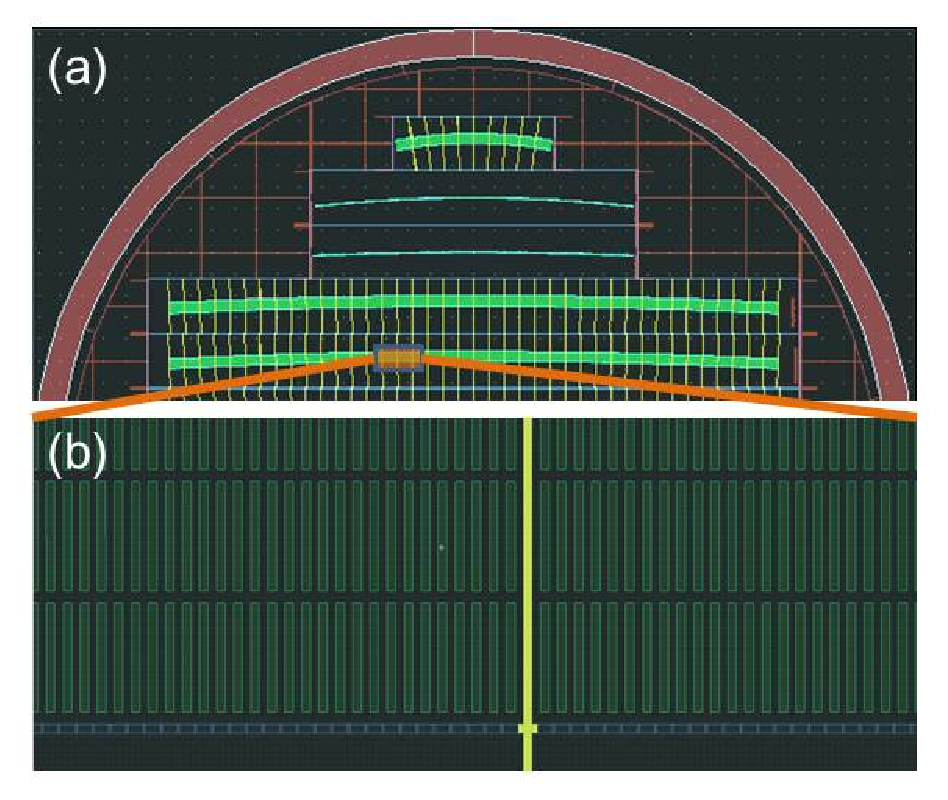
\includegraphics[width=.6\textwidth]{figures/grating_mask.eps}
    \caption{Grating design mask for
        the edge-on illumination approach and \ac{SEM}
        image of the grating. The top part of the 4 inch wafer shows
        five grating chips. The
        gratings have different curvatures which are specific to the grating
        interferometer geometry. 
        The \ac{SEM} image shows the gold structures and the interrupting bridges
        that prevent the lamellae from collapsing~\cite{Kenntner2010}.}
        \label{Fig:grating_mask}
\end{figure}

Due to the high spectral acceptance~\cite{Weitkamp2005,Thuering2013c} of the
interferometer ($\SI{50}{\kilo\electronvolt}$ to
more than $\SI{160}{\kilo\electronvolt}$) and the high attenuation efficiencies of
the source and analyzer gratings ($>90\%$ up to
$\SI{160}{\kilo\electronvolt}$), the voltage of the X-ray source was set to
the maximum of $\SI{160}{\kilo\volt}$. With a grating structure height of
approximately $\SI{100}{\micro \metre}$, the field of view in the vertical
direction is limited to one detector pixel row. In the horizontal direction,
the field of view is only limited by the grating size to
$\SI{30}{\milli\metre}$, but wider gratings can be fabricated with this
method and the available technology on larger wafers. In addition to the standard components (source,
camera, interferometer), two optical slits, one in front of the source
grating, the other in front of the camera, were required for the collimation
of the beam in the vertical direction. 

Fig.~\ref{Fig:img_chip} shows a radiographic scan of an electronic chip.
Several resistors and an integrated circuits are located on different layers
on the chip. The images were acquired in scanning mode, using a step size of
$\SI{100}{\micro \metre}$ along the $y$ axis. For a better comparison of the
magnified phase and attenuation images, the attenuation image has been
replaced with the differential attenuation image, which was obtained by
digital differentiation. In the attenuation image, the contrast of the soldering points of
the integrated circuit is reduced underneath the resistors, while in
the phase image, they can clearly be identified. The reduced contrast of the 
soldering points in the absorption image is due to beam hardening. The spectrum
impinging on these soldering point is hardened by the resistors in the upper
layer, resulting in lower absorption contrast. Due to the weaker energy
dependency of phase shifts ($1/E$ compared to $1/E^3$), phase-contrast images
are less sensitive to beam hardening~\cite{Chabior2011a}, which explains the
lower contrast reduction of the soldering points underneath the resistors in the
phase image of the chip. This result shows the benefit of the phase nature in
high-energy X-ray imaging, which may be useful to identify flaws in multilayered
structures such as electronic chips.
\begin{figure}[ht]
    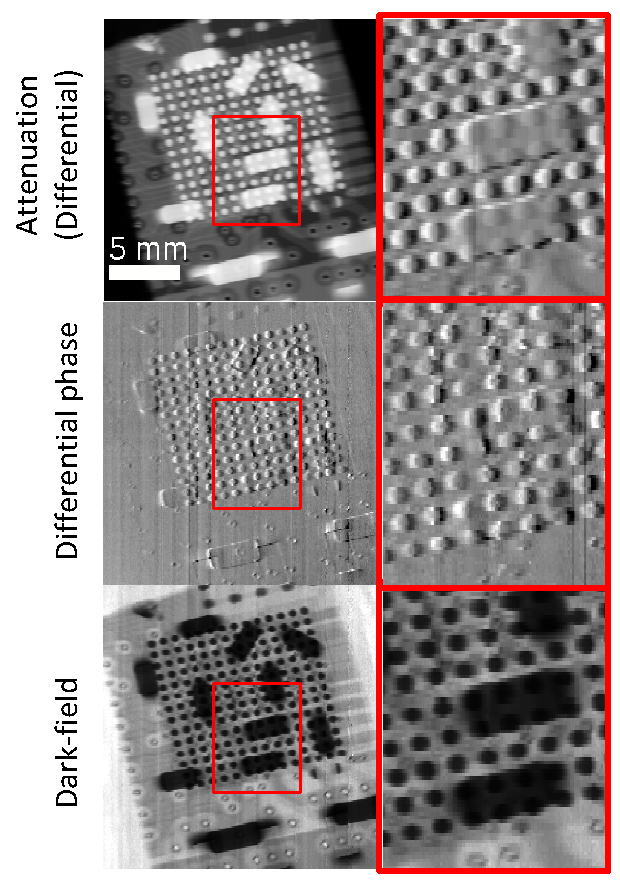
\includegraphics[width=.5\textwidth]{figures/img_chip_dabs.eps}
    \caption{Radiographic scan of an electronic chip. The image was acquired
        with 24 phase steps per line and an exposure time of \SI{15}{\second} per
    step. The top right image shows the differential absorption image.}
    \label{Fig:img_chip}
\end{figure}

Edge-on illuminated grating interferometry finally allows phase contrast
imaging to be performed at high energies ($>\SI{100}{\kilo\eV}$) on conventional X-ray
sources. With a circular distribution of the gratings, the diffracting and
absorbing structures can be matched to the divergent beam, even for very
compact geometries. Short, high-energy phase-contrast systems enable the
efficient investigation of high-density materials or large thickness,
adding information on electron density and integrated small angle scattering
power to the conventional absorption based signal. This will improve
material discrimination and density sensitivity capabilities in future
X-rays or even neutron~\cite{Grunzweig2008} investigations.

\section*{Methods}
Edge-on illuminated gratings were manufactured by Microworks GmbH, Germany, using a LIGA process~\cite{Kenntner2010}. Each grating
resides on a $5 \times \SI{60}{\milli\metre^2}$ silicon chip and several
grating chips are fabricated on a single 4 inch silicon wafer. The
experimental arrangement for a design energy at \SI{100}{\kilo\electronvolt}
is a symmetric Talbot-Lau interferometer with a grating period of $p =
\SI{2.8}{\micro \metre}$ for all gratings. The distance from the source
grating to the analyzer grating is $\SI{32}{\centi\metre}$ and the source
grating is positioned $\SI{23}{\centi\metre}$ away from the source.

The X-ray source is a COMET MXR-160HP/11 X-ray tube with a maximum output
voltage of $\SI{160}{\kilo\volt}$. In the experiment, it was set to the
maximum voltage. The focal spot size is approximately
$\SI{1}{\milli\metre}$. The detector is a CCD camera from Finger Lakes
Instruments. A cesium iodide (CsI:Ti) scintillator of $\SI{600}{\micro
\metre}$ thickness converts the X-rays to visible light and is coupled with
an optical lens projecting the image onto the CCD. The effective pixel size
is $\SI{80}{\micro \metre}$. The widths of the collimating slits are
$\SI{25}{\micro \metre}$ and $\SI{100}{\micro\metre}$, respectively.

In Fig.~\ref{Fig:img_chip}, image acquisition involved 24 phase steps per
line and an exposure time of 15 seconds per step. The long
exposure times are mostly constrained by the low average visibility of the
gratings (\SI{5}{\percent}). The exposure time was chosen in order to
get a low noise in the differential phase image. The \ac{SNR} is
proportional to the visibility and the square root of the exposure
time~\cite{Raupach2011}.
This implies that the exposure times can easily drop by an order of
magnitude as these gratings become comparable in quality to those developed
in the last ten years. 
Smaller regions of these gratings actually exhibit a visibility up
to~\SI{14}{\percent} already, indicating that this goal is reachable as the
fabrication becomes more reliable and uniform.
The detector is also relatively inefficient ($\approx \SI{30}{\percent})$
leaving an additional margin for improvement.



\section*{Acknowledgements}
We thank Gordan Mikuljan, Peter Modregger and István Mohácsi from the Paul
Scherrer Institute (PSI), Switzerland, for the
work on the mechanical design, the scientific advice, and the \ac{SEM} images
respectively, Joachim Schulz and Marco Walter from
Microworks GmbH, Germany, for the competent support on grating design
issues, Christian Kottler and Vincent Revol from Centre Suisse
d'Electronique et de Microtechnique (CSEM), Switzerland for the fruitful
discussions on the design of the system. This work has been partially
supported by the Competence Centre for Materials Science and Technology
(CCMX) of the ETH Board, Project Nr. 61 and by the ERC Grant ERC-2012-StG 310005-PhaseX.

\bibliographystyle{apsrev4-1}
%\bibliography{library}

%merlin.mbs apsrev4-1.bst 2010-07-25 4.21a (PWD, AO, DPC) hacked
%Control: key (0)
%Control: author (72) initials jnrlst
%Control: editor formatted (1) identically to author
%Control: production of article title (-1) disabled
%Control: page (0) single
%Control: year (1) truncated
%Control: production of eprint (0) enabled
\begin{thebibliography}{33}%
\makeatletter
\providecommand \@ifxundefined [1]{%
 \@ifx{#1\undefined}
}%
\providecommand \@ifnum [1]{%
 \ifnum #1\expandafter \@firstoftwo
 \else \expandafter \@secondoftwo
 \fi
}%
\providecommand \@ifx [1]{%
 \ifx #1\expandafter \@firstoftwo
 \else \expandafter \@secondoftwo
 \fi
}%
\providecommand \natexlab [1]{#1}%
\providecommand \enquote  [1]{``#1''}%
\providecommand \bibnamefont  [1]{#1}%
\providecommand \bibfnamefont [1]{#1}%
\providecommand \citenamefont [1]{#1}%
\providecommand \href@noop [0]{\@secondoftwo}%
\providecommand \href [0]{\begingroup \@sanitize@url \@href}%
\providecommand \@href[1]{\@@startlink{#1}\@@href}%
\providecommand \@@href[1]{\endgroup#1\@@endlink}%
\providecommand \@sanitize@url [0]{\catcode `\\12\catcode `\$12\catcode
  `\&12\catcode `\#12\catcode `\^12\catcode `\_12\catcode `\%12\relax}%
\providecommand \@@startlink[1]{}%
\providecommand \@@endlink[0]{}%
\providecommand \url  [0]{\begingroup\@sanitize@url \@url }%
\providecommand \@url [1]{\endgroup\@href {#1}{\urlprefix }}%
\providecommand \urlprefix  [0]{URL }%
\providecommand \Eprint [0]{\href }%
\providecommand \doibase [0]{http://dx.doi.org/}%
\providecommand \selectlanguage [0]{\@gobble}%
\providecommand \bibinfo  [0]{\@secondoftwo}%
\providecommand \bibfield  [0]{\@secondoftwo}%
\providecommand \translation [1]{[#1]}%
\providecommand \BibitemOpen [0]{}%
\providecommand \bibitemStop [0]{}%
\providecommand \bibitemNoStop [0]{.\EOS\space}%
\providecommand \EOS [0]{\spacefactor3000\relax}%
\providecommand \BibitemShut  [1]{\csname bibitem#1\endcsname}%
\let\auto@bib@innerbib\@empty
%</preamble>
\bibitem [{\citenamefont {Als-Nielsen}\ and\ \citenamefont
  {McMorrow}(2011)}]{Als-Nielsen2011}%
  \BibitemOpen
  \bibfield  {author} {\bibinfo {author} {\bibfnamefont {J.}~\bibnamefont
  {Als-Nielsen}}\ and\ \bibinfo {author} {\bibfnamefont {D.}~\bibnamefont
  {McMorrow}},\ }\href
  {http://books.google.com/books?hl=en\&lr=\&id=rlqlboWlTRMC\&oi=fnd\&pg=PA29\&dq=Elements+of+Modern+X-ray+Physics\&ots=P2D3XwrDgd\&sig=b3iO97q1hfsT8TkTYKxsvUbFink}
  {\emph {\bibinfo {title} {{Elements of modern X-ray physics}}}}\ (\bibinfo
  {year} {2011})\BibitemShut {NoStop}%
\bibitem [{\citenamefont {Qi}\ \emph {et~al.}(2010)\citenamefont {Qi},
  \citenamefont {Zambelli}, \citenamefont {Bevins},\ and\ \citenamefont
  {Chen}}]{Qi2010}%
  \BibitemOpen
  \bibfield  {author} {\bibinfo {author} {\bibfnamefont {Z.}~\bibnamefont
  {Qi}}, \bibinfo {author} {\bibfnamefont {J.}~\bibnamefont {Zambelli}},
  \bibinfo {author} {\bibfnamefont {N.}~\bibnamefont {Bevins}}, \ and\ \bibinfo
  {author} {\bibfnamefont {G.-H.}\ \bibnamefont {Chen}},\ }\href {\doibase
  10.1088/0031-9155/55/9/016} {\bibfield  {journal} {\bibinfo  {journal}
  {Physics in medicine and biology}\ }\textbf {\bibinfo {volume} {55}},\
  \bibinfo {pages} {2669} (\bibinfo {year} {2010})}\BibitemShut {NoStop}%
\bibitem [{\citenamefont {Pfeiffer}\ \emph {et~al.}(2007)\citenamefont
  {Pfeiffer}, \citenamefont {Bunk}, \citenamefont {David}, \citenamefont
  {Bech}, \citenamefont {{Le Duc}}, \citenamefont {Bravin},\ and\ \citenamefont
  {Cloetens}}]{Pfeiffer2007a}%
  \BibitemOpen
  \bibfield  {author} {\bibinfo {author} {\bibfnamefont {F.}~\bibnamefont
  {Pfeiffer}}, \bibinfo {author} {\bibfnamefont {O.}~\bibnamefont {Bunk}},
  \bibinfo {author} {\bibfnamefont {C.}~\bibnamefont {David}}, \bibinfo
  {author} {\bibfnamefont {M.}~\bibnamefont {Bech}}, \bibinfo {author}
  {\bibfnamefont {G.}~\bibnamefont {{Le Duc}}}, \bibinfo {author}
  {\bibfnamefont {A.}~\bibnamefont {Bravin}}, \ and\ \bibinfo {author}
  {\bibfnamefont {P.}~\bibnamefont {Cloetens}},\ }\href {\doibase
  10.1088/0031-9155/52/23/010} {\bibfield  {journal} {\bibinfo  {journal}
  {Physics in medicine and biology}\ }\textbf {\bibinfo {volume} {52}},\
  \bibinfo {pages} {6923} (\bibinfo {year} {2007})}\BibitemShut {NoStop}%
\bibitem [{\citenamefont {McDonald}\ \emph {et~al.}(2009)\citenamefont
  {McDonald}, \citenamefont {Marone}, \citenamefont {Hintermuller},
  \citenamefont {Mikuljan}, \citenamefont {David}, \citenamefont {Pfeiffer},
  \citenamefont {Stampanoni},\ and\ \citenamefont
  {Hinterm\"{u}ller}}]{McDonald2009}%
  \BibitemOpen
  \bibfield  {author} {\bibinfo {author} {\bibfnamefont {S.~A.}\ \bibnamefont
  {McDonald}}, \bibinfo {author} {\bibfnamefont {F.}~\bibnamefont {Marone}},
  \bibinfo {author} {\bibfnamefont {C.}~\bibnamefont {Hintermuller}}, \bibinfo
  {author} {\bibfnamefont {G.}~\bibnamefont {Mikuljan}}, \bibinfo {author}
  {\bibfnamefont {C.}~\bibnamefont {David}}, \bibinfo {author} {\bibfnamefont
  {F.}~\bibnamefont {Pfeiffer}}, \bibinfo {author} {\bibfnamefont
  {M.}~\bibnamefont {Stampanoni}}, \ and\ \bibinfo {author} {\bibfnamefont
  {C.}~\bibnamefont {Hinterm\"{u}ller}},\ }\href {\doibase
  10.1107/S0909049509017920} {\bibfield  {journal} {\bibinfo  {journal}
  {Journal of Synchrotron Radiation}\ }\textbf {\bibinfo {volume} {16}},\
  \bibinfo {pages} {562} (\bibinfo {year} {2009})}\BibitemShut {NoStop}%
\bibitem [{\citenamefont {Davis}\ \emph {et~al.}(1995)\citenamefont {Davis},
  \citenamefont {Gao}, \citenamefont {Gureyev}, \citenamefont {Stevenson},\
  and\ \citenamefont {Wilkins}}]{Davis1995}%
  \BibitemOpen
  \bibfield  {author} {\bibinfo {author} {\bibfnamefont {T.}~\bibnamefont
  {Davis}}, \bibinfo {author} {\bibfnamefont {D.}~\bibnamefont {Gao}}, \bibinfo
  {author} {\bibfnamefont {T.}~\bibnamefont {Gureyev}}, \bibinfo {author}
  {\bibfnamefont {A.}~\bibnamefont {Stevenson}}, \ and\ \bibinfo {author}
  {\bibfnamefont {S.}~\bibnamefont {Wilkins}},\ }\href
  {http://imaging.sbes.vt.edu/laboratory/XGI/(1995 Gao).pdf} {\bibfield
  {journal} {\bibinfo  {journal} {Nature}\ }\textbf {\bibinfo {volume} {373}},\
  \bibinfo {pages} {595} (\bibinfo {year} {1995})}\BibitemShut {NoStop}%
\bibitem [{\citenamefont {Chapman}\ \emph {et~al.}(1997)\citenamefont
  {Chapman}, \citenamefont {Thomlinson}, \citenamefont {Johnston},
  \citenamefont {Washburn}, \citenamefont {Pisano}, \citenamefont {Gm\"{u}r},
  \citenamefont {Zhong}, \citenamefont {Menk}, \citenamefont {Arfelli},\ and\
  \citenamefont {Sayers}}]{Chapman1997}%
  \BibitemOpen
  \bibfield  {author} {\bibinfo {author} {\bibfnamefont {D.}~\bibnamefont
  {Chapman}}, \bibinfo {author} {\bibfnamefont {W.}~\bibnamefont {Thomlinson}},
  \bibinfo {author} {\bibfnamefont {R.}~\bibnamefont {Johnston}}, \bibinfo
  {author} {\bibfnamefont {D.}~\bibnamefont {Washburn}}, \bibinfo {author}
  {\bibfnamefont {E.}~\bibnamefont {Pisano}}, \bibinfo {author} {\bibfnamefont
  {N.}~\bibnamefont {Gm\"{u}r}}, \bibinfo {author} {\bibfnamefont
  {Z.}~\bibnamefont {Zhong}}, \bibinfo {author} {\bibfnamefont
  {R.}~\bibnamefont {Menk}}, \bibinfo {author} {\bibfnamefont {F.}~\bibnamefont
  {Arfelli}}, \ and\ \bibinfo {author} {\bibfnamefont {D.}~\bibnamefont
  {Sayers}},\ }\href {\doibase 10.1016/j.carj.2010.04.015} {\bibfield
  {journal} {\bibinfo  {journal} {Physics in Medicine and Biology}\ }\textbf
  {\bibinfo {volume} {42}},\ \bibinfo {pages} {2015} (\bibinfo {year}
  {1997})}\BibitemShut {NoStop}%
\bibitem [{\citenamefont {Bonse}\ and\ \citenamefont {Hart}(1965)}]{Bonse1965}%
  \BibitemOpen
  \bibfield  {author} {\bibinfo {author} {\bibfnamefont {U.}~\bibnamefont
  {Bonse}}\ and\ \bibinfo {author} {\bibfnamefont {M.}~\bibnamefont {Hart}},\
  }\href {http://link.aip.org/link/?APPLAB/6/155/1} {\bibfield  {journal}
  {\bibinfo  {journal} {Applied Physics Letters}\ }\textbf {\bibinfo {volume}
  {6}},\ \bibinfo {pages} {155} (\bibinfo {year} {1965})}\BibitemShut {NoStop}%
\bibitem [{\citenamefont {Momose}\ \emph {et~al.}(1996)\citenamefont {Momose},
  \citenamefont {Takeda}, \citenamefont {Itai},\ and\ \citenamefont
  {Hirano}}]{Momose1996}%
  \BibitemOpen
  \bibfield  {author} {\bibinfo {author} {\bibfnamefont {A.}~\bibnamefont
  {Momose}}, \bibinfo {author} {\bibfnamefont {T.}~\bibnamefont {Takeda}},
  \bibinfo {author} {\bibfnamefont {Y.}~\bibnamefont {Itai}}, \ and\ \bibinfo
  {author} {\bibfnamefont {K.}~\bibnamefont {Hirano}},\ }\href
  {http://imaging.sbes.vt.edu/laboratory/XGI/(1996 Momose).pdf} {\bibfield
  {journal} {\bibinfo  {journal} {Nature Medicine}\ }\textbf {\bibinfo {volume}
  {2}},\ \bibinfo {pages} {473} (\bibinfo {year} {1996})}\BibitemShut {NoStop}%
\bibitem [{\citenamefont {Snigirev}\ \emph {et~al.}(1995)\citenamefont
  {Snigirev}, \citenamefont {Snigireva}, \citenamefont {Kohn}, \citenamefont
  {Kuznetsov},\ and\ \citenamefont {Schelokov}}]{Snigirev1995}%
  \BibitemOpen
  \bibfield  {author} {\bibinfo {author} {\bibfnamefont {A.}~\bibnamefont
  {Snigirev}}, \bibinfo {author} {\bibfnamefont {I.}~\bibnamefont {Snigireva}},
  \bibinfo {author} {\bibfnamefont {V.}~\bibnamefont {Kohn}}, \bibinfo {author}
  {\bibfnamefont {S.}~\bibnamefont {Kuznetsov}}, \ and\ \bibinfo {author}
  {\bibfnamefont {I.}~\bibnamefont {Schelokov}},\ }\href
  {http://kohnvict.narod.ru/articles/091.pdf} {\bibfield  {journal} {\bibinfo
  {journal} {Review of Scientific Instruments}\ }\textbf {\bibinfo {volume}
  {66}},\ \bibinfo {pages} {5486} (\bibinfo {year} {1995})}\BibitemShut
  {NoStop}%
\bibitem [{\citenamefont {Wilkins}\ \emph {et~al.}(1996)\citenamefont
  {Wilkins}, \citenamefont {Gureyev}, \citenamefont {Gao}, \citenamefont
  {Pogany},\ and\ \citenamefont {Stevenson}}]{Wilkins1996}%
  \BibitemOpen
  \bibfield  {author} {\bibinfo {author} {\bibfnamefont {S.}~\bibnamefont
  {Wilkins}}, \bibinfo {author} {\bibfnamefont {T.}~\bibnamefont {Gureyev}},
  \bibinfo {author} {\bibfnamefont {D.}~\bibnamefont {Gao}}, \bibinfo {author}
  {\bibfnamefont {A.}~\bibnamefont {Pogany}}, \ and\ \bibinfo {author}
  {\bibfnamefont {A.}~\bibnamefont {Stevenson}},\ }\href
  {http://fisica.ufpr.br/lorxi/Rcf2/artigos/Wilkins.pdf} {\bibfield  {journal}
  {\bibinfo  {journal} {Nature}\ }\textbf {\bibinfo {volume} {384}},\ \bibinfo
  {pages} {335} (\bibinfo {year} {1996})}\BibitemShut {NoStop}%
\bibitem [{\citenamefont {Cloetens}\ \emph {et~al.}(1996)\citenamefont
  {Cloetens}, \citenamefont {Barrett}, \citenamefont {Baruchel}, \citenamefont
  {Guigay},\ and\ \citenamefont {Schlenker}}]{Cloetens1996}%
  \BibitemOpen
  \bibfield  {author} {\bibinfo {author} {\bibfnamefont {P.}~\bibnamefont
  {Cloetens}}, \bibinfo {author} {\bibfnamefont {R.}~\bibnamefont {Barrett}},
  \bibinfo {author} {\bibfnamefont {J.}~\bibnamefont {Baruchel}}, \bibinfo
  {author} {\bibfnamefont {J.}~\bibnamefont {Guigay}}, \ and\ \bibinfo {author}
  {\bibfnamefont {M.}~\bibnamefont {Schlenker}},\ }\href
  {http://iopscience.iop.org/0022-3727/29/1/023} {\bibfield  {journal}
  {\bibinfo  {journal} {Journal of Physics D: Applied Physics}\ }\textbf
  {\bibinfo {volume} {29}},\ \bibinfo {pages} {133} (\bibinfo {year}
  {1996})}\BibitemShut {NoStop}%
\bibitem [{\citenamefont {Cloetens}\ \emph {et~al.}(1997)\citenamefont
  {Cloetens}, \citenamefont {Guigay}, \citenamefont {{De Martino}},
  \citenamefont {Baruchel},\ and\ \citenamefont {Schlenker}}]{Cloetens1997}%
  \BibitemOpen
  \bibfield  {author} {\bibinfo {author} {\bibfnamefont {P.}~\bibnamefont
  {Cloetens}}, \bibinfo {author} {\bibfnamefont {J.}~\bibnamefont {Guigay}},
  \bibinfo {author} {\bibfnamefont {C.}~\bibnamefont {{De Martino}}}, \bibinfo
  {author} {\bibfnamefont {J.}~\bibnamefont {Baruchel}}, \ and\ \bibinfo
  {author} {\bibfnamefont {M.}~\bibnamefont {Schlenker}},\ }\href
  {http://www.ncbi.nlm.nih.gov/pubmed/18185750} {\bibfield  {journal} {\bibinfo
   {journal} {Optics letters}\ }\textbf {\bibinfo {volume} {22}},\ \bibinfo
  {pages} {1059} (\bibinfo {year} {1997})}\BibitemShut {NoStop}%
\bibitem [{\citenamefont {David}\ \emph {et~al.}(2002)\citenamefont {David},
  \citenamefont {N\"{o}hammer}, \citenamefont {Solak},\ and\ \citenamefont
  {Ziegler}}]{David2002}%
  \BibitemOpen
  \bibfield  {author} {\bibinfo {author} {\bibfnamefont {C.}~\bibnamefont
  {David}}, \bibinfo {author} {\bibfnamefont {B.}~\bibnamefont {N\"{o}hammer}},
  \bibinfo {author} {\bibfnamefont {H.}~\bibnamefont {Solak}}, \ and\ \bibinfo
  {author} {\bibfnamefont {E.}~\bibnamefont {Ziegler}},\ }\href {\doibase
  10.1063/1.1516611} {\bibfield  {journal} {\bibinfo  {journal} {Applied
  Physics Letters}\ }\textbf {\bibinfo {volume} {81}},\ \bibinfo {pages} {3287}
  (\bibinfo {year} {2002})}\BibitemShut {NoStop}%
\bibitem [{\citenamefont {Momose}\ \emph {et~al.}(2003)\citenamefont {Momose},
  \citenamefont {Kawamoto}, \citenamefont {Koyama}, \citenamefont {Hamaishi},
  \citenamefont {Takai},\ and\ \citenamefont {Suzuki}}]{Momose2003a}%
  \BibitemOpen
  \bibfield  {author} {\bibinfo {author} {\bibfnamefont {A.}~\bibnamefont
  {Momose}}, \bibinfo {author} {\bibfnamefont {S.}~\bibnamefont {Kawamoto}},
  \bibinfo {author} {\bibfnamefont {I.}~\bibnamefont {Koyama}}, \bibinfo
  {author} {\bibfnamefont {Y.}~\bibnamefont {Hamaishi}}, \bibinfo {author}
  {\bibfnamefont {K.}~\bibnamefont {Takai}}, \ and\ \bibinfo {author}
  {\bibfnamefont {Y.}~\bibnamefont {Suzuki}},\ }\href {\doibase
  10.1143/JJAP.42.L866} {\bibfield  {journal} {\bibinfo  {journal} {Japanese
  Journal of Applied Physics}\ }\textbf {\bibinfo {volume} {42}},\ \bibinfo
  {pages} {L866} (\bibinfo {year} {2003})}\BibitemShut {NoStop}%
\bibitem [{\citenamefont {Munro}\ \emph {et~al.}(2012)\citenamefont {Munro},
  \citenamefont {Ignatyev}, \citenamefont {Speller},\ and\ \citenamefont
  {Olivo}}]{Munro2012}%
  \BibitemOpen
  \bibfield  {author} {\bibinfo {author} {\bibfnamefont {P.}~\bibnamefont
  {Munro}}, \bibinfo {author} {\bibfnamefont {K.}~\bibnamefont {Ignatyev}},
  \bibinfo {author} {\bibfnamefont {R.}~\bibnamefont {Speller}}, \ and\
  \bibinfo {author} {\bibfnamefont {A.}~\bibnamefont {Olivo}},\ }\href
  {\doibase 10.1073/pnas.1205396109} {\bibfield  {journal} {\bibinfo  {journal}
  {Proceedings of the National Academy of Sciences}\ }\textbf {\bibinfo
  {volume} {2012}},\ \bibinfo {pages} {2} (\bibinfo {year} {2012})}\BibitemShut
  {NoStop}%
\bibitem [{\citenamefont {Pfeiffer}\ \emph {et~al.}(2006)\citenamefont
  {Pfeiffer}, \citenamefont {Weitkamp}, \citenamefont {Bunk},\ and\
  \citenamefont {David}}]{Pfeiffer2006}%
  \BibitemOpen
  \bibfield  {author} {\bibinfo {author} {\bibfnamefont {F.}~\bibnamefont
  {Pfeiffer}}, \bibinfo {author} {\bibfnamefont {T.}~\bibnamefont {Weitkamp}},
  \bibinfo {author} {\bibfnamefont {O.}~\bibnamefont {Bunk}}, \ and\ \bibinfo
  {author} {\bibfnamefont {C.}~\bibnamefont {David}},\ }\href {\doibase
  10.1038/nphys265} {\bibfield  {journal} {\bibinfo  {journal} {Nature
  Physics}\ }\textbf {\bibinfo {volume} {2}},\ \bibinfo {pages} {258} (\bibinfo
  {year} {2006})}\BibitemShut {NoStop}%
\bibitem [{\citenamefont {Nesch}\ \emph {et~al.}(2009)\citenamefont {Nesch},
  \citenamefont {Fogarty}, \citenamefont {Tzvetkov}, \citenamefont {Reinhart},
  \citenamefont {Walus}, \citenamefont {Khelashvili}, \citenamefont
  {Muehleman},\ and\ \citenamefont {Chapman}}]{Nesch2009}%
  \BibitemOpen
  \bibfield  {author} {\bibinfo {author} {\bibfnamefont {I.}~\bibnamefont
  {Nesch}}, \bibinfo {author} {\bibfnamefont {D.~P.}\ \bibnamefont {Fogarty}},
  \bibinfo {author} {\bibfnamefont {T.}~\bibnamefont {Tzvetkov}}, \bibinfo
  {author} {\bibfnamefont {B.}~\bibnamefont {Reinhart}}, \bibinfo {author}
  {\bibfnamefont {a.~C.}\ \bibnamefont {Walus}}, \bibinfo {author}
  {\bibfnamefont {G.}~\bibnamefont {Khelashvili}}, \bibinfo {author}
  {\bibfnamefont {C.}~\bibnamefont {Muehleman}}, \ and\ \bibinfo {author}
  {\bibfnamefont {D.}~\bibnamefont {Chapman}},\ }\href {\doibase
  10.1063/1.3213621} {\bibfield  {journal} {\bibinfo  {journal} {The Review of
  scientific instruments}\ }\textbf {\bibinfo {volume} {80}},\ \bibinfo {pages}
  {093702} (\bibinfo {year} {2009})}\BibitemShut {NoStop}%
\bibitem [{\citenamefont {Parham}\ \emph {et~al.}(2009)\citenamefont {Parham},
  \citenamefont {Zhong}, \citenamefont {Connor}, \citenamefont {Chapman},\ and\
  \citenamefont {Pisano}}]{Parham2009}%
  \BibitemOpen
  \bibfield  {author} {\bibinfo {author} {\bibfnamefont {C.}~\bibnamefont
  {Parham}}, \bibinfo {author} {\bibfnamefont {Z.}~\bibnamefont {Zhong}},
  \bibinfo {author} {\bibfnamefont {D.~M.}\ \bibnamefont {Connor}}, \bibinfo
  {author} {\bibfnamefont {L.~D.}\ \bibnamefont {Chapman}}, \ and\ \bibinfo
  {author} {\bibfnamefont {E.~D.}\ \bibnamefont {Pisano}},\ }\href
  {http://linkinghub.elsevier.com/retrieve/pii/S1076633209001366?showall=true}
  {\enquote {\bibinfo {title} {{Design and Implementation of a Compact Low-Dose
  Diffraction Enhanced Medical Imaging System}},}\ } (\bibinfo {year}
  {2009})\BibitemShut {NoStop}%
\bibitem [{\citenamefont {Pfeiffer}\ \emph {et~al.}(2008)\citenamefont
  {Pfeiffer}, \citenamefont {Bech}, \citenamefont {Bunk}, \citenamefont
  {Kraft}, \citenamefont {Eikenberry}, \citenamefont {Br\"{o}nnimann},
  \citenamefont {Gr\"{u}nzweig},\ and\ \citenamefont {David}}]{Pfeiffer2008}%
  \BibitemOpen
  \bibfield  {author} {\bibinfo {author} {\bibfnamefont {F.}~\bibnamefont
  {Pfeiffer}}, \bibinfo {author} {\bibfnamefont {M.}~\bibnamefont {Bech}},
  \bibinfo {author} {\bibfnamefont {O.}~\bibnamefont {Bunk}}, \bibinfo {author}
  {\bibfnamefont {P.}~\bibnamefont {Kraft}}, \bibinfo {author} {\bibfnamefont
  {E.}~\bibnamefont {Eikenberry}}, \bibinfo {author} {\bibfnamefont
  {C.}~\bibnamefont {Br\"{o}nnimann}}, \bibinfo {author} {\bibfnamefont
  {C.}~\bibnamefont {Gr\"{u}nzweig}}, \ and\ \bibinfo {author} {\bibfnamefont
  {C.}~\bibnamefont {David}},\ }\href {\doibase 10.1038/nmat2096} {\bibfield
  {journal} {\bibinfo  {journal} {Nature Materials}\ }\textbf {\bibinfo
  {volume} {7}},\ \bibinfo {pages} {134} (\bibinfo {year} {2008})}\BibitemShut
  {NoStop}%
\bibitem [{\citenamefont {Willner}\ \emph {et~al.}(2013)\citenamefont
  {Willner}, \citenamefont {Bech}, \citenamefont {Herzen}, \citenamefont
  {Zanette}, \citenamefont {Hahn}, \citenamefont {Kenntner}, \citenamefont
  {Mohr}, \citenamefont {Rack}, \citenamefont {Weitkamp},\ and\ \citenamefont
  {Pfeiffer}}]{Willner2013}%
  \BibitemOpen
  \bibfield  {author} {\bibinfo {author} {\bibfnamefont {M.}~\bibnamefont
  {Willner}}, \bibinfo {author} {\bibfnamefont {M.}~\bibnamefont {Bech}},
  \bibinfo {author} {\bibfnamefont {J.}~\bibnamefont {Herzen}}, \bibinfo
  {author} {\bibfnamefont {I.}~\bibnamefont {Zanette}}, \bibinfo {author}
  {\bibfnamefont {D.}~\bibnamefont {Hahn}}, \bibinfo {author} {\bibfnamefont
  {J.}~\bibnamefont {Kenntner}}, \bibinfo {author} {\bibfnamefont
  {J.}~\bibnamefont {Mohr}}, \bibinfo {author} {\bibfnamefont {A.}~\bibnamefont
  {Rack}}, \bibinfo {author} {\bibfnamefont {T.}~\bibnamefont {Weitkamp}}, \
  and\ \bibinfo {author} {\bibfnamefont {F.}~\bibnamefont {Pfeiffer}},\ }\href
  {http://www.ncbi.nlm.nih.gov/pubmed/23481949} {\bibfield  {journal} {\bibinfo
   {journal} {Optics express}\ }\textbf {\bibinfo {volume} {21}},\ \bibinfo
  {pages} {4155} (\bibinfo {year} {2013})}\BibitemShut {NoStop}%
\bibitem [{\citenamefont {Ruiz}\ \emph {et~al.}(2013)\citenamefont {Ruiz},
  \citenamefont {Zanette}, \citenamefont {Chabior}, \citenamefont {Scherer},
  \citenamefont {Mohr}, \citenamefont {Walter}, \citenamefont {Weitkamp},
  \citenamefont {Rack},\ and\ \citenamefont {Pfeiffer}}]{Ruiz2013}%
  \BibitemOpen
  \bibfield  {author} {\bibinfo {author} {\bibfnamefont {M.}~\bibnamefont
  {Ruiz}}, \bibinfo {author} {\bibfnamefont {I.}~\bibnamefont {Zanette}},
  \bibinfo {author} {\bibfnamefont {M.}~\bibnamefont {Chabior}}, \bibinfo
  {author} {\bibfnamefont {K.}~\bibnamefont {Scherer}}, \bibinfo {author}
  {\bibfnamefont {J.}~\bibnamefont {Mohr}}, \bibinfo {author} {\bibfnamefont
  {M.}~\bibnamefont {Walter}}, \bibinfo {author} {\bibfnamefont
  {T.}~\bibnamefont {Weitkamp}}, \bibinfo {author} {\bibfnamefont
  {A.}~\bibnamefont {Rack}}, \ and\ \bibinfo {author} {\bibfnamefont
  {F.}~\bibnamefont {Pfeiffer}},\ }\href@noop {} {\bibfield  {journal}
  {\bibinfo  {journal} {Poster, 2nd International Symposium on BioMedical
  Applications of X-ray Phase Contrast Imaging, Germany, 24/25th January 2013}\
  } (\bibinfo {year} {2013})}\BibitemShut {NoStop}%
\bibitem [{\citenamefont {Donath}\ \emph {et~al.}(2009)\citenamefont {Donath},
  \citenamefont {Chabior}, \citenamefont {Pfeiffer}, \citenamefont {Bunk},
  \citenamefont {Reznikova}, \citenamefont {Mohr}, \citenamefont {Hempel},
  \citenamefont {Popescu}, \citenamefont {Hoheisel}, \citenamefont {Schuster},
  \citenamefont {Baumann},\ and\ \citenamefont {David}}]{Donath2009}%
  \BibitemOpen
  \bibfield  {author} {\bibinfo {author} {\bibfnamefont {T.}~\bibnamefont
  {Donath}}, \bibinfo {author} {\bibfnamefont {M.}~\bibnamefont {Chabior}},
  \bibinfo {author} {\bibfnamefont {F.}~\bibnamefont {Pfeiffer}}, \bibinfo
  {author} {\bibfnamefont {O.}~\bibnamefont {Bunk}}, \bibinfo {author}
  {\bibfnamefont {E.}~\bibnamefont {Reznikova}}, \bibinfo {author}
  {\bibfnamefont {J.}~\bibnamefont {Mohr}}, \bibinfo {author} {\bibfnamefont
  {E.}~\bibnamefont {Hempel}}, \bibinfo {author} {\bibfnamefont
  {S.}~\bibnamefont {Popescu}}, \bibinfo {author} {\bibfnamefont
  {M.}~\bibnamefont {Hoheisel}}, \bibinfo {author} {\bibfnamefont
  {M.}~\bibnamefont {Schuster}}, \bibinfo {author} {\bibfnamefont
  {J.}~\bibnamefont {Baumann}}, \ and\ \bibinfo {author} {\bibfnamefont
  {C.}~\bibnamefont {David}},\ }\href {\doibase 10.1063/1.3208052} {\bibfield
  {journal} {\bibinfo  {journal} {Journal of Applied Physics}\ }\textbf
  {\bibinfo {volume} {106}},\ \bibinfo {pages} {054703} (\bibinfo {year}
  {2009})}\BibitemShut {NoStop}%
\bibitem [{\citenamefont {Mohr}\ \emph {et~al.}(2012)\citenamefont {Mohr},
  \citenamefont {Grund}, \citenamefont {Kunka}, \citenamefont {Kenntner},
  \citenamefont {Leuthold}, \citenamefont {Meiser}, \citenamefont {Schulz},\
  and\ \citenamefont {Walter}}]{Mohr2012}%
  \BibitemOpen
  \bibfield  {author} {\bibinfo {author} {\bibfnamefont {J.}~\bibnamefont
  {Mohr}}, \bibinfo {author} {\bibfnamefont {T.}~\bibnamefont {Grund}},
  \bibinfo {author} {\bibfnamefont {D.}~\bibnamefont {Kunka}}, \bibinfo
  {author} {\bibfnamefont {J.}~\bibnamefont {Kenntner}}, \bibinfo {author}
  {\bibfnamefont {J.}~\bibnamefont {Leuthold}}, \bibinfo {author}
  {\bibfnamefont {J.}~\bibnamefont {Meiser}}, \bibinfo {author} {\bibfnamefont
  {J.}~\bibnamefont {Schulz}}, \ and\ \bibinfo {author} {\bibfnamefont
  {M.}~\bibnamefont {Walter}},\ }\href {\doibase 10.1063/1.4742267} {\ \textbf
  {\bibinfo {volume} {41}},\ \bibinfo {pages} {41} (\bibinfo {year}
  {2012})}\BibitemShut {NoStop}%
\bibitem [{\citenamefont {David}\ \emph {et~al.}(2007)\citenamefont {David},
  \citenamefont {Bruder}, \citenamefont {Rohbeck}, \citenamefont
  {Gr\"{u}nzweig}, \citenamefont {Kottler}, \citenamefont {Diaz}, \citenamefont
  {Bunk},\ and\ \citenamefont {Pfeiffer}}]{David2007}%
  \BibitemOpen
  \bibfield  {author} {\bibinfo {author} {\bibfnamefont {C.}~\bibnamefont
  {David}}, \bibinfo {author} {\bibfnamefont {J.}~\bibnamefont {Bruder}},
  \bibinfo {author} {\bibfnamefont {T.}~\bibnamefont {Rohbeck}}, \bibinfo
  {author} {\bibfnamefont {C.}~\bibnamefont {Gr\"{u}nzweig}}, \bibinfo {author}
  {\bibfnamefont {C.}~\bibnamefont {Kottler}}, \bibinfo {author} {\bibfnamefont
  {A.}~\bibnamefont {Diaz}}, \bibinfo {author} {\bibfnamefont {O.}~\bibnamefont
  {Bunk}}, \ and\ \bibinfo {author} {\bibfnamefont {F.}~\bibnamefont
  {Pfeiffer}},\ }\href {\doibase 10.1016/j.mee.2007.01.151} {\bibfield
  {journal} {\bibinfo  {journal} {Microelectronic Engineering}\ }\textbf
  {\bibinfo {volume} {84}},\ \bibinfo {pages} {1172} (\bibinfo {year}
  {2007})}\BibitemShut {NoStop}%
\bibitem [{\citenamefont {Kenntner}\ \emph {et~al.}(2010)\citenamefont
  {Kenntner}, \citenamefont {Grund}, \citenamefont {Matthis}, \citenamefont
  {Boerner}, \citenamefont {Mohr}, \citenamefont {Scherer}, \citenamefont
  {Walter}, \citenamefont {Willner}, \citenamefont {Tapfer}, \citenamefont
  {Bech}, \citenamefont {Pfeiffer}, \citenamefont {Zanette},\ and\
  \citenamefont {Weitkamp}}]{Kenntner2010}%
  \BibitemOpen
  \bibfield  {author} {\bibinfo {author} {\bibfnamefont {J.}~\bibnamefont
  {Kenntner}}, \bibinfo {author} {\bibfnamefont {T.}~\bibnamefont {Grund}},
  \bibinfo {author} {\bibfnamefont {B.}~\bibnamefont {Matthis}}, \bibinfo
  {author} {\bibfnamefont {M.}~\bibnamefont {Boerner}}, \bibinfo {author}
  {\bibfnamefont {J.}~\bibnamefont {Mohr}}, \bibinfo {author} {\bibfnamefont
  {T.}~\bibnamefont {Scherer}}, \bibinfo {author} {\bibfnamefont
  {M.}~\bibnamefont {Walter}}, \bibinfo {author} {\bibfnamefont
  {M.}~\bibnamefont {Willner}}, \bibinfo {author} {\bibfnamefont
  {A.}~\bibnamefont {Tapfer}}, \bibinfo {author} {\bibfnamefont
  {M.}~\bibnamefont {Bech}}, \bibinfo {author} {\bibfnamefont {F.}~\bibnamefont
  {Pfeiffer}}, \bibinfo {author} {\bibfnamefont {I.}~\bibnamefont {Zanette}}, \
  and\ \bibinfo {author} {\bibfnamefont {T.}~\bibnamefont {Weitkamp}},\ }in\
  \href@noop {} {\emph {\bibinfo {booktitle} {Proceedings of SPIE}}},\ Vol.\
  \bibinfo {volume} {7804}\ (\bibinfo {year} {2010})\ p.\ \bibinfo {pages}
  {780408}\BibitemShut {NoStop}%
\bibitem [{\citenamefont {Stutman}\ and\ \citenamefont
  {Finkenthal}(2012)}]{Stutman2012a}%
  \BibitemOpen
  \bibfield  {author} {\bibinfo {author} {\bibfnamefont {D.}~\bibnamefont
  {Stutman}}\ and\ \bibinfo {author} {\bibfnamefont {M.}~\bibnamefont
  {Finkenthal}},\ }\href {\doibase 10.1063/1.4748882} {\bibfield  {journal}
  {\bibinfo  {journal} {Applied physics letters}\ }\textbf {\bibinfo {volume}
  {101}},\ \bibinfo {pages} {91108} (\bibinfo {year} {2012})}\BibitemShut
  {NoStop}%
\bibitem [{\citenamefont {{\AA slund, M}}(2007)}]{Aslund2007}%
  \BibitemOpen
  \bibfield  {author} {\bibinfo {author} {\bibnamefont {{\AA slund, M}}},\
  }\emph {\bibinfo {title} {{Digital Mammography with a Photon Counting
  Detector in a Scanned Multislit Geometry}}},\ \href@noop {} {Ph.D. thesis}
  (\bibinfo {year} {2007})\BibitemShut {NoStop}%
\bibitem [{\citenamefont {Oduko}\ \emph {et~al.}(2010)\citenamefont {Oduko},
  \citenamefont {Young},\ and\ \citenamefont {Burch}}]{Oduko2010}%
  \BibitemOpen
  \bibfield  {author} {\bibinfo {author} {\bibfnamefont {J.~M.}\ \bibnamefont
  {Oduko}}, \bibinfo {author} {\bibfnamefont {K.~C.}\ \bibnamefont {Young}}, \
  and\ \bibinfo {author} {\bibfnamefont {A.}~\bibnamefont {Burch}},\ }in\ \href
  {\doibase 10.1007/978-3-642-13666-5_49} {\emph {\bibinfo {booktitle} {Digital
  Mammography}}},\ \bibinfo {series} {Lecture Notes in Computer Science}, Vol.\
  \bibinfo {volume} {6136},\ \bibinfo {editor} {edited by\ \bibinfo {editor}
  {\bibfnamefont {J.}~\bibnamefont {Martí}}, \bibinfo {editor} {\bibfnamefont
  {A.}~\bibnamefont {Oliver}}, \bibinfo {editor} {\bibfnamefont
  {J.}~\bibnamefont {Freixenet}}, \ and\ \bibinfo {editor} {\bibfnamefont
  {R.}~\bibnamefont {Martí}}}\ (\bibinfo  {publisher} {Springer Berlin
  Heidelberg},\ \bibinfo {year} {2010})\ pp.\ \bibinfo {pages}
  {365--370}\BibitemShut {NoStop}%
\bibitem [{\citenamefont {Weitkamp}\ \emph {et~al.}(2005)\citenamefont
  {Weitkamp}, \citenamefont {Diaz}, \citenamefont {David}, \citenamefont
  {Pfeiffer}, \citenamefont {Stampanoni}, \citenamefont {Cloetens},\ and\
  \citenamefont {Ziegler}}]{Weitkamp2005}%
  \BibitemOpen
  \bibfield  {author} {\bibinfo {author} {\bibfnamefont {T.}~\bibnamefont
  {Weitkamp}}, \bibinfo {author} {\bibfnamefont {A.}~\bibnamefont {Diaz}},
  \bibinfo {author} {\bibfnamefont {C.}~\bibnamefont {David}}, \bibinfo
  {author} {\bibfnamefont {F.}~\bibnamefont {Pfeiffer}}, \bibinfo {author}
  {\bibfnamefont {M.}~\bibnamefont {Stampanoni}}, \bibinfo {author}
  {\bibfnamefont {P.}~\bibnamefont {Cloetens}}, \ and\ \bibinfo {author}
  {\bibfnamefont {E.}~\bibnamefont {Ziegler}},\ }\href {\doibase
  10.1364/OPEX.13.006296} {\bibfield  {journal} {\bibinfo  {journal} {Optics
  Express}\ }\textbf {\bibinfo {volume} {13}},\ \bibinfo {pages} {6296}
  (\bibinfo {year} {2005})}\BibitemShut {NoStop}%
\bibitem [{\citenamefont {Thuering}\ \emph {et~al.}(2013)\citenamefont
  {Thuering}, \citenamefont {Barber}, \citenamefont {Seo}, \citenamefont
  {Alhassen}, \citenamefont {Iwanczyk},\ and\ \citenamefont
  {Stampanoni}}]{Thuering2013c}%
  \BibitemOpen
  \bibfield  {author} {\bibinfo {author} {\bibfnamefont {T.}~\bibnamefont
  {Thuering}}, \bibinfo {author} {\bibfnamefont {W.}~\bibnamefont {Barber}},
  \bibinfo {author} {\bibfnamefont {Y.}~\bibnamefont {Seo}}, \bibinfo {author}
  {\bibfnamefont {F.}~\bibnamefont {Alhassen}}, \bibinfo {author}
  {\bibfnamefont {J.}~\bibnamefont {Iwanczyk}}, \ and\ \bibinfo {author}
  {\bibfnamefont {M.}~\bibnamefont {Stampanoni}},\ }\href {\doibase
  10.1063/1.4805073} {\bibfield  {journal} {\bibinfo  {journal} {Applied
  Physics Letters}\ }\textbf {\bibinfo {volume} {102}},\ \bibinfo {pages}
  {191113} (\bibinfo {year} {2013})}\BibitemShut {NoStop}%
\bibitem [{\citenamefont {Chabior}\ \emph {et~al.}(2011)\citenamefont
  {Chabior}, \citenamefont {Donath}, \citenamefont {David}, \citenamefont
  {Bunk}, \citenamefont {Schuster}, \citenamefont {Schroer},\ and\
  \citenamefont {Pfeiffer}}]{Chabior2011a}%
  \BibitemOpen
  \bibfield  {author} {\bibinfo {author} {\bibfnamefont {M.}~\bibnamefont
  {Chabior}}, \bibinfo {author} {\bibfnamefont {T.}~\bibnamefont {Donath}},
  \bibinfo {author} {\bibfnamefont {C.}~\bibnamefont {David}}, \bibinfo
  {author} {\bibfnamefont {O.}~\bibnamefont {Bunk}}, \bibinfo {author}
  {\bibfnamefont {M.}~\bibnamefont {Schuster}}, \bibinfo {author}
  {\bibfnamefont {C.}~\bibnamefont {Schroer}}, \ and\ \bibinfo {author}
  {\bibfnamefont {F.}~\bibnamefont {Pfeiffer}},\ }\href {\doibase
  10.1118/1.3553408} {\bibfield  {journal} {\bibinfo  {journal} {Medical
  Physics}\ }\textbf {\bibinfo {volume} {38}},\ \bibinfo {pages} {1189}
  (\bibinfo {year} {2011})}\BibitemShut {NoStop}%
\bibitem [{\citenamefont {Gr\"{u}nzweig}\ \emph {et~al.}(2008)\citenamefont
  {Gr\"{u}nzweig}, \citenamefont {Pfeiffer}, \citenamefont {Bunk},
  \citenamefont {Donath}, \citenamefont {K\"{u}hne}, \citenamefont {Frei},
  \citenamefont {Dierolf},\ and\ \citenamefont {David}}]{Grunzweig2008}%
  \BibitemOpen
  \bibfield  {author} {\bibinfo {author} {\bibfnamefont {C.}~\bibnamefont
  {Gr\"{u}nzweig}}, \bibinfo {author} {\bibfnamefont {F.}~\bibnamefont
  {Pfeiffer}}, \bibinfo {author} {\bibfnamefont {O.}~\bibnamefont {Bunk}},
  \bibinfo {author} {\bibfnamefont {T.}~\bibnamefont {Donath}}, \bibinfo
  {author} {\bibfnamefont {G.}~\bibnamefont {K\"{u}hne}}, \bibinfo {author}
  {\bibfnamefont {G.}~\bibnamefont {Frei}}, \bibinfo {author} {\bibfnamefont
  {M.}~\bibnamefont {Dierolf}}, \ and\ \bibinfo {author} {\bibfnamefont
  {C.}~\bibnamefont {David}},\ }\href {\doibase 10.1063/1.2930866} {\bibfield
  {journal} {\bibinfo  {journal} {The Review of scientific instruments}\
  }\textbf {\bibinfo {volume} {79}},\ \bibinfo {pages} {053703} (\bibinfo
  {year} {2008})}\BibitemShut {NoStop}%
\bibitem [{\citenamefont {Raupach}\ and\ \citenamefont
  {Flohr}(2011)}]{Raupach2011}%
  \BibitemOpen
  \bibfield  {author} {\bibinfo {author} {\bibfnamefont {R.}~\bibnamefont
  {Raupach}}\ and\ \bibinfo {author} {\bibfnamefont {T.~G.}\ \bibnamefont
  {Flohr}},\ }\href {\doibase 10.1088/0031-9155/56/7/020} {\bibfield  {journal}
  {\bibinfo  {journal} {Physics in medicine and biology}\ }\textbf {\bibinfo
  {volume} {56}},\ \bibinfo {pages} {2219} (\bibinfo {year}
  {2011})}\BibitemShut {NoStop}%
\end{thebibliography}%
\end{document}
